\section{Motivating Example}
\label{sec:motivation}

This section motivates {\grafter} using an example based on Apache Ant. The change scenario is constructed by us to illustrate the difficulty of catching cloning bugs. Figure~\ref{fig:example} shows the pair of inconsistently edited clones, one from the {\ttt setIncludes} method in the {\ttt Copy} class (lines 6-15 in Figure~\ref{fig:example}a) and the other from the {\ttt setExcludes} method in the {\ttt Delete} class (lines 6-15 in Figure~\ref{fig:example}b). These clones are syntactically similar but not identical---the left program uses a field {\ttt includes} of type {\ttt IncludePatternSet} while the right program uses a field {\ttt excludes} of type {\ttt ExcludePatternSet}. The {\ttt Copy} class implements the task of copying files matching the specified file pattern(s). On the other hand, {\ttt Delete} removes files that do not match the pattern(s). Methods {\ttt setIncludes} and {\ttt setExcludes} both split the input string by a comma and add each pattern to a pattern set, {\ttt includes} and {\ttt excludes} respectively. Figure~\ref{fig:test} shows a test case, {\ttt testCopy}, which creates a {\ttt Copy} object, specifies two copied file patterns as a string {\ttt "src/*.java, test/*.java"}, and then checks if all java files in the {\ttt src} folder and the {\ttt test} folder are copied to a target directory. However, the {\ttt Delete} class is not tested by any existing test. 

%\begin{figure}[!t]
%\centering
%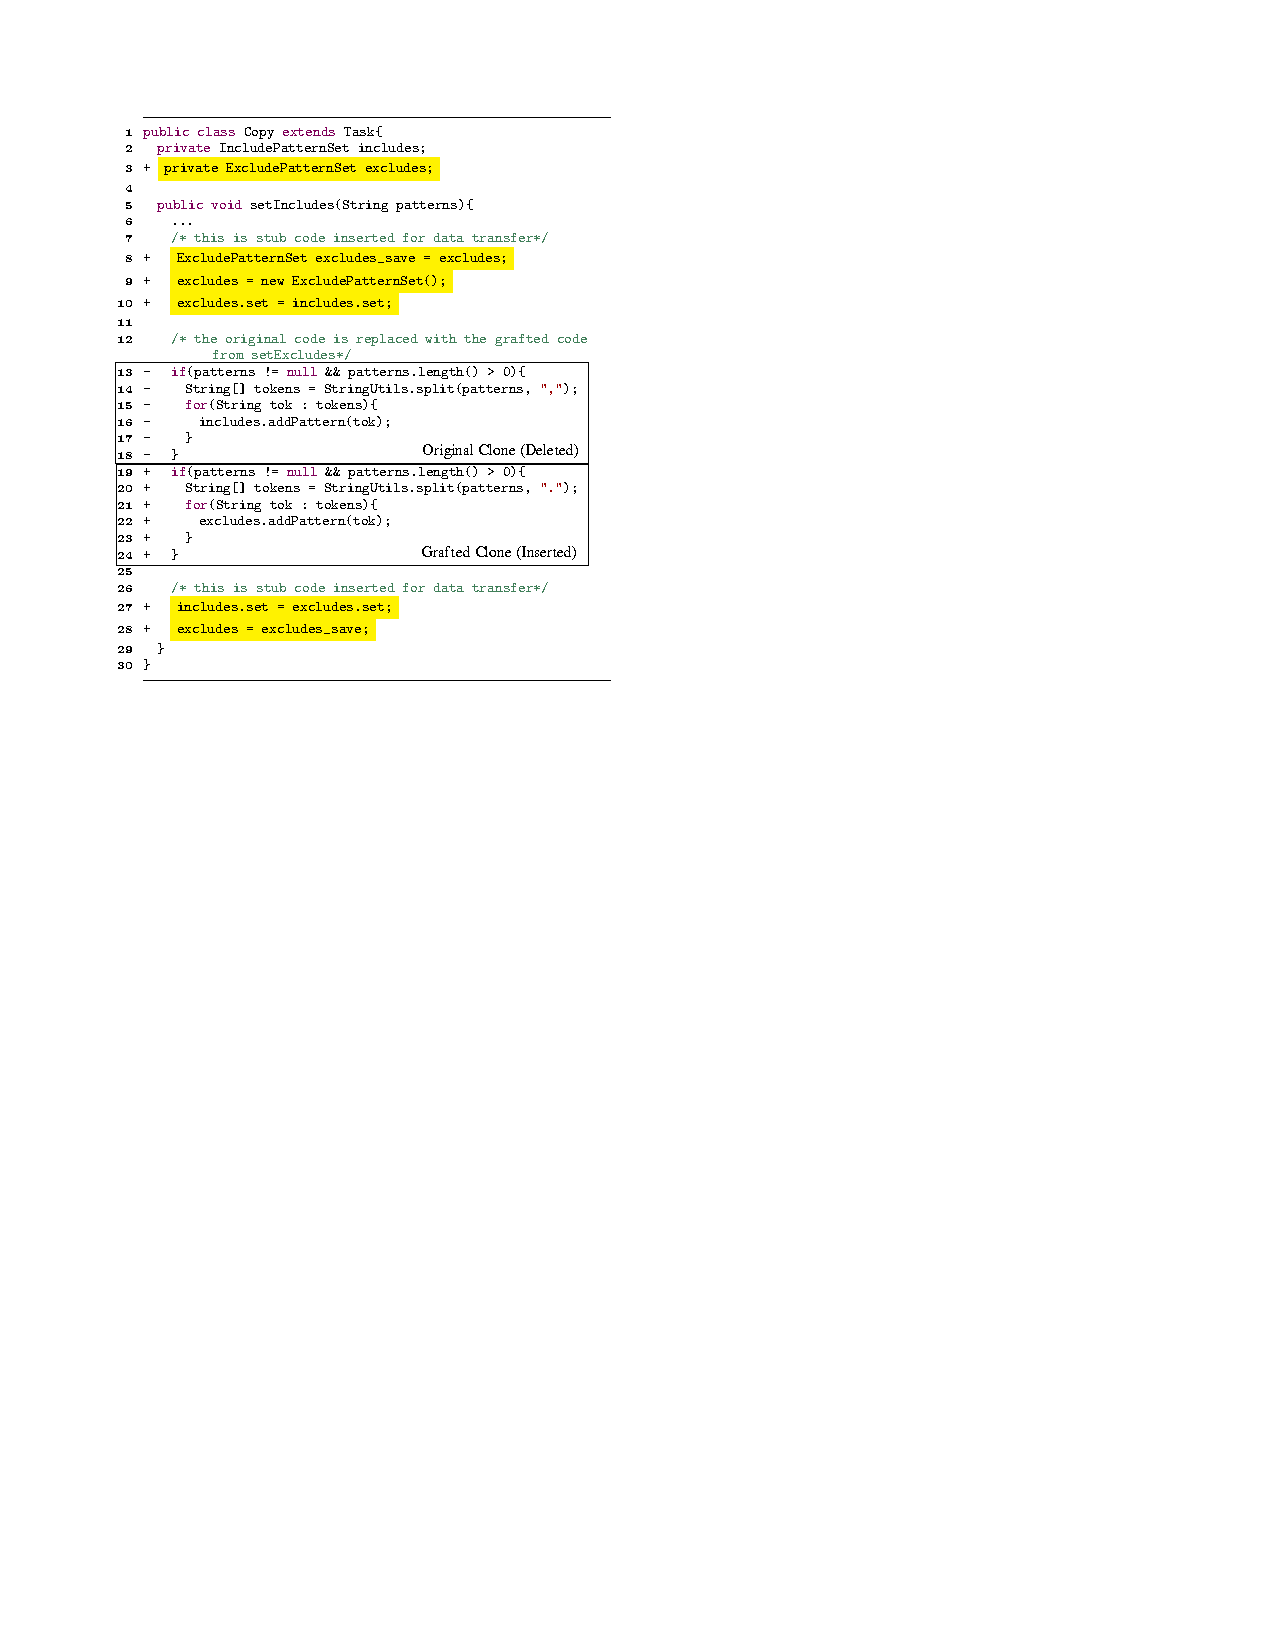
\includegraphics[width=0.45\textwidth]{graftedcode.pdf}
%\caption{{\grafter} grafts the clone in {\ttt Delete} (lines 19-24) in place of the original clone in {\ttt Copy} (lines 13-18) for test reuse. {\grafter} inserts stub code (highlighted in yellow).}
%\label{fig:output}
%\vspace{-4mm}
%\end{figure}

{\ttt StringTokenizer} is a legacy class and its usage is now discouraged in new code. Therefore, Alice updates the use of {\ttt StringTokenizer} API to {\ttt StringUtils.split} in both {\ttt Copy} and {\ttt Delete} in Figure~\ref{fig:example}. However, she accidentally changes the separator from {\ttt `,'} to {\ttt `.'}~in {\ttt Delete} (line 11 in Figure~\ref{fig:example}b). Such mistake is difficult to notice during manual inspection, as these programs are similar but not identical. An existing cloning bug finder by Jiang et al.~would fail to find the mistake, as it checks for only three pre-defined cloning bug types via static analysis~\cite{Jiang2007}: renaming mistakes, control construct inconsistency, and conditional predicate inconsistency. Accidentally replacing the separator does not belong to any of the pre-defined cloning bug types.

{\bf Inspect clones.} Alice can inspect clones by right clicking a clone group and select ``Compare''. Each clone in the group is named in the format of ``(start line number, end line number)'' by default. Alice can double-click and rename a clone, but it has to be in the format of ``XYZ(start line number, end line number)''. Grafter automatically excludes trivial clone groups (e.g., clones in test files) and mark them in red. If Alice believes Grafter mistakenly filters out a clone group, Alice can re-add this group by right-clicking on it and select "Include". When inspecting clones, you can discard a clone group by right-click -> Exclude. Alice can click ``Export'' and save all clone groups of interest to an xml file. All excluded clones will be discarded and not exported to the xml file.

{\bf Find test cases for clones.} Alice does not need to specify the test cases. Instead, Alice can just click the ``Coverage'' button and {\grafter} will automatically locate test cases for each clone. This is very helpful when Alice is investigating a large code base with a large number of test cases.

{\bf Reuse test and examine behavior differences.} {\grafter} supports the behavior comparison in two granularities. Alice can compare the test outcomes of two clones by right-clicking the clone group and selecting ``Compare Test Behavior''. The comparison results are represented in a table and behavioral differences are highlighted in red for ease of investigation. The first column shows names of test cases. The second and third columns show whether each clone passes or fails the corresponding test case. The last column shows the comparison result. Green means both clones are consistent on this test and red means their test outcomes are different.

Alice can also compare the intermediate state values of two clones by right-clicking the clone group and selecting ``Compare State Behavior''. In the state-level comparison table, the first and third columns show the name of corresponding variables referenced by code clones, and the second and fourth columns show the values of variables in the format of XML. Grafter prints the value of an object in XML using XStream.

To reuse the same test {\ttt testCopy} for {\ttt Delete}, {\grafter} grafts the clone from {\ttt Delete} in place of the original clone in {\ttt Copy}, as shown in Figure~\ref{fig:output}. As the grafted code uses an undefined variable {\ttt excludes}, {\grafter} also ports its declaration to {\ttt Copy.java}. {\grafter} ensures that the grafted clone receives the same input data by populating {\ttt excludes} with the value of {\ttt includes} (lines 8-10) and transfers the value of {\ttt excludes} back to {\ttt includes} (lines 27-28). Therefore, the value of {\ttt excludes} can flow into the same assertion check of the original test. Additional stub code generated by {\grafter} is highlighted in yellow in Figure~\ref{fig:output}.

After grafting, {\grafter} runs {\ttt testCopy} on both clones and finds that the test now fails on {\ttt Delete}, because the string is not split properly. To help Alice further diagnose failure symptoms, {\grafter} shows that {\ttt tokens} has a list \{ {\ttt "src/*.java"}, {\ttt "test/*.java"}\} in {\ttt Copy} but \{ {\ttt "src/*"}, {\ttt "java, test/*"}, {\ttt "java"} \} in {\ttt Delete} due to a wrong split. {\grafter} also shows that this difference has propagated to corresponding variables {\ttt includes} and {\ttt excludes}.